\section{Các thành phần và sơ đồ đấu nối}
\subsection{Các thành phần}
\subsubsection{Relay trung gian}
\begin{itemize}
    \item \textbf{Cấu tạo relay trung gian:} Relay trung gian được cấu tạo gồm 2 bộ phận: Nam châm điện cùng hệ thống các tiếp điểm đóng ngắt 
    , được dùng rất nhiều trong ngành điện tử, điện công nghiệp \dots
    \begin{itemize}
        \item Nam châm điện: Được thiết kế gồm: lõi thép động, lõi thép tĩnh, cuộn dây
        (cuộn dây cường độ, cuộn điện áp hoặc cả 2). Lõi thép động được định vị bằng vít điều chỉnh, và găng bằng lò xo. 
        \item Mạch tiếp điểm. 
    \end{itemize}
    \item \textbf{Nguyên lý hoạt động:} Dòng điện chạy qua relay trung gian sẽ chạy qua cuộn dây bên trong và tạo ra một từ trường hút. Tác động lên đòn bẩy bên trong làm đóng hoặc mở các tiếp điểm điện. Trạng thái của relay được thay đổi, số tiếp điểm bị
    thay đổi 1 chiều hoặc nhiều chiều phụ thuộc vào thiết kế.
    \begin{figure}[H]
        \centering
        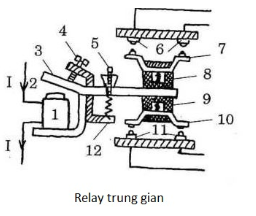
\includegraphics[width=0.5\textwidth]{pictures/NLHD_relay.png}
    \end{figure}
    \item Relay trung gian MY4N AC240/250, 14 chân, 5A (4PDT)
    \begin{figure}[H]
        \centering
        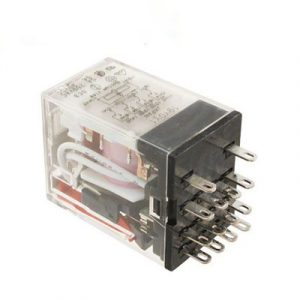
\includegraphics[width=0.5\textwidth]{pictures/Relay_4PDT.png}
    \end{figure}
    \item Relay trung gian MY2N AC240/250, 8 chân, 5A (DPDT)
    \begin{figure}[H]
        \centering
        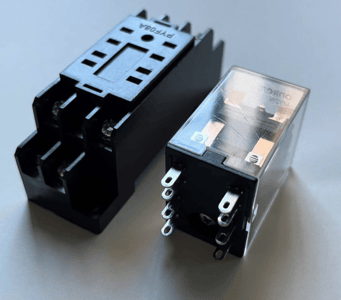
\includegraphics[width=0.5\textwidth]{pictures/Relay_DPDT.png}
    \end{figure}
\end{itemize}

\subsubsection{Module relay 4 kênh}
Module relay được sử dụng chung với cảm biến phát hiện kim loại. 
\begin{figure}[H]
    \centering
    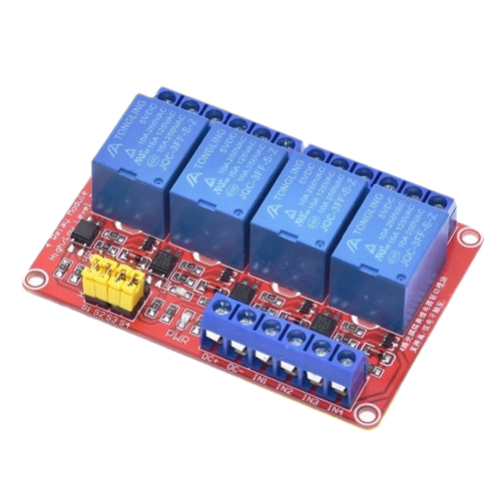
\includegraphics[width=0.5\textwidth]{pictures/Module_relay.png}
\end{figure}



\subsubsection{Cảm biến tiệm cận kim loại}
\begin{itemize}
    \item Cảm biến tiệm cận (Proximity Sensors). Còn có tên gọi khác là công tắc tiệm cận
    hay "PROX". Phản ứng khi có vật ở gần cảm biến.
    \item \textbf{Nguyên lý hoạt động:} Cảm biến tiệm cận NPN hoạt động dựa trên nguyên lý của 
    transitor NPN. Cấu tạo của cảm biến tiệm cận bao gồm 1 mạch phát hiện vật, mục đích để xử lí tín hiệu
    khi phát hiện vật gần cảm biến và chuyển đổi thành tín hiện điện cho mạch kế tiếp. Tiếp theo là 1 mạch ON/OFF NPN sử dụng tín hiệu
    điện từ mạch phát hiện vật để đóng ngắt transistor. Cuối cùng tín hiệu được xuất ra ngoài output (Output có thể là PLC, relay hoặc tải, \dots)
    \begin{figure}[H]
        \centering
        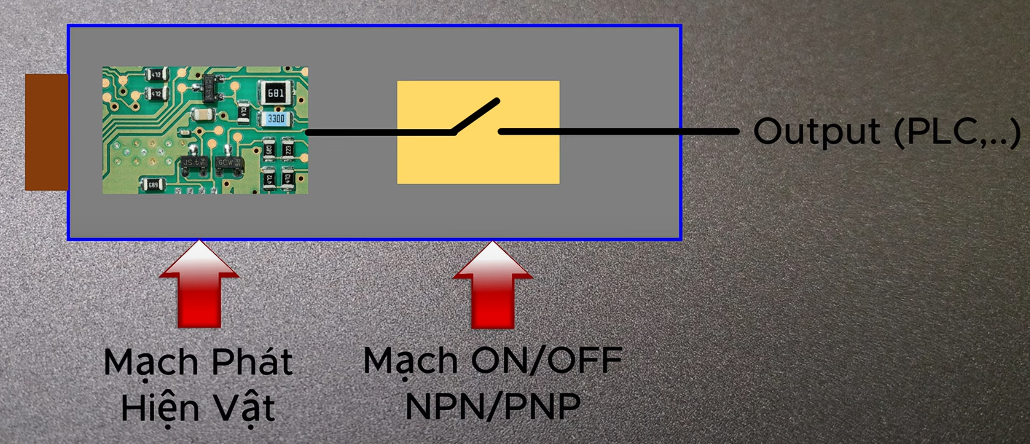
\includegraphics[width=0.7\textwidth]{pictures/structure_sensor.png}
    \end{figure}
    Cách đấu nối dây cho mạch sử dụng cảm biến tiệm cận kim loại NPN:
    \begin{figure}[H]
        \centering
        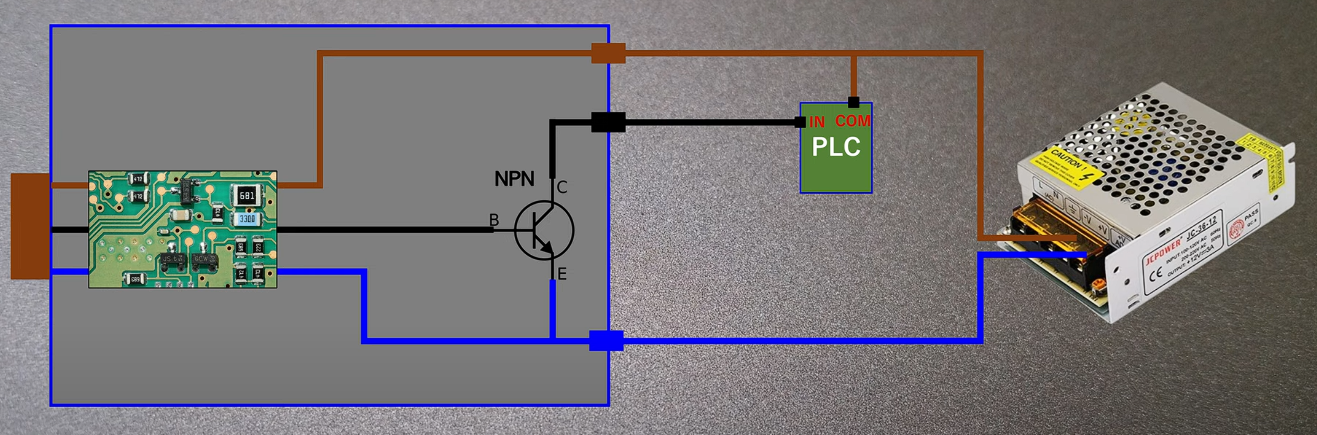
\includegraphics[width=1\textwidth]{pictures/mach_sensor.png}
    \end{figure}
    Trong trường hợp ở đây, chân tín hiệu của cảm biến sẽ được kết nối với module relay nhằm thực hiện nhiệm vụ như 1 công tắc trong mạch điều khiển
    ở các vị trí A1, B1, A2, B2.
\end{itemize}
Cảm biến phát hiện kim loại LJ12A3 loại NPN. 
\begin{figure}[H]
    \centering
    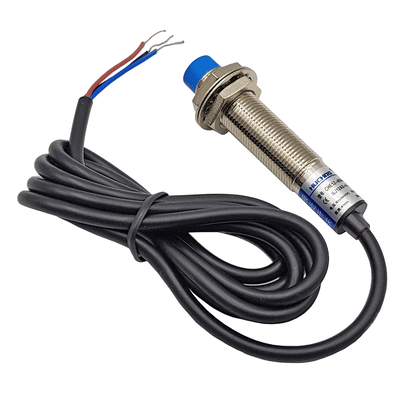
\includegraphics[width=0.5\textwidth]{pictures/Sensor.png}
\end{figure}
\cleardoublepage



\subsubsection{Động cơ}
Động cơ giảm tốc hộp số vuông góc JGY370 18RPM
\begin{figure}[H]
    \centering
    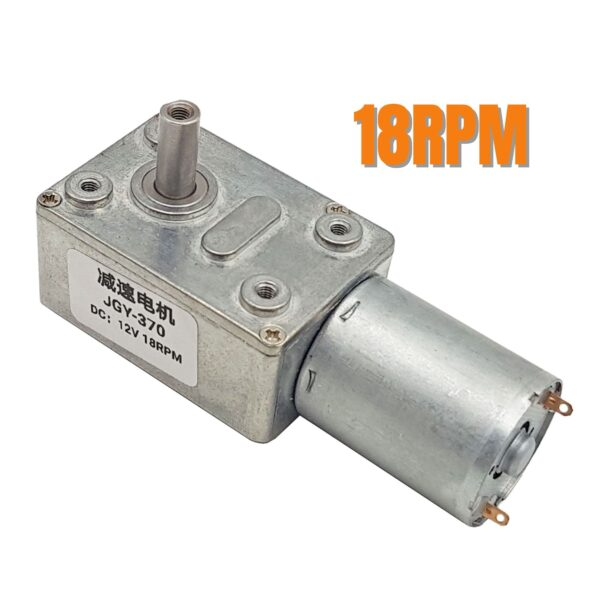
\includegraphics[width=0.5\textwidth]{pictures/motor.png}
\end{figure}

\cleardoublepage